\documentclass{article}
\usepackage[a4paper]{geometry}
\usepackage[utf8]{inputenc}
\usepackage{graphicx}
\usepackage{makecell}
\usepackage{amsmath}
\usepackage{listings}
\usepackage{xcolor}
\usepackage{animate}
\usepackage{subcaption}

\title{Data Mining Project\\CN2 Algorithm for Rules Induction}
\author{Paolo Baldini}
\date{\today}

\begin{document}

\maketitle
\newpage

%%%%%%%%%%%%%%%%%%%%%%%%%%%%%%%%%%%%%%%%%%%%%%%%%%%%%%%%%%%%%%%%%%%%%%%%%%%%%%%%%%%%%%%%%%%%%%%%%%%
% ABSTRACT
%%%%%%%%%%%%%%%%%%%%%%%%%%%%%%%%%%%%%%%%%%%%%%%%%%%%%%%%%%%%%%%%%%%%%%%%%%%%%%%%%%%%%%%%%%%%%%%%%%%

\section*{Abstract - Description of the task}
The aim of the project is the implementation of a data mining algorithm. A testing of its properties (scaling, influence of parameters values on results) is also required.
\vspace{12pt}\newline
The algorithm implementation and analysis that will be treated in this report regard the CN2 rules induction algorithm presented by Clark and Niblett during the eighties.
\vspace{12pt}\newline
The test of the algorithm will use the original datasets evaluated by Clark and Niblett in their paper. These are the \textit{Breast Cancer}, \textit{Lymphography} and \textit{Primary Tumor} datasets from the University Medical Centre, Institute of Oncology, Ljubljana, Yugoslavia.
\newpage

\tableofcontents
\newpage

%%%%%%%%%%%%%%%%%%%%%%%%%%%%%%%%%%%%%%%%%%%%%%%%%%%%%%%%%%%%%%%%%%%%%%%%%%%%%%%%%%%%%%%%%%%%%%%%%%%
% SECTION 1
%%%%%%%%%%%%%%%%%%%%%%%%%%%%%%%%%%%%%%%%%%%%%%%%%%%%%%%%%%%%%%%%%%%%%%%%%%%%%%%%%%%%%%%%%%%%%%%%%%%

\section{Objectives and testing}
The objective of this project is the implementation of the data mining CN2 algorithm for the induction of decision lists made of classification rules. The algorithm has been proposed by Clark and Niblett at the end of the eighties. From now on, we will refer to the two researcher with the abbreviation `C\&N'.
\vspace{12pt}\newline
The implementation will be done in the Kotlin programming language running on the JVM.
\vspace{12pt}\newline
To evaluate the implementation and the inferred rules, I chose to repeat the tests carried out by C\&N during the writing of their paper.\newline
This method of evaluation is possible in that the original datasets used by C\&N are still available on the internet and guarantee a directly comparison for the performance of the algorithm.\newline
The testing of the algorithm's properties will then be conducted evaluating its performance at the change of the parameters with the above mentioned datasets.\newline
To avoid wrong evaluations by a possible overfitting of the rules, the evaluation will use training and test sets with homogeneously distributed classes.
\vspace{12pt}\newline
For more information about the used datasets and testing methods please refer to Section \ref{section:tests}.
\newpage

%%%%%%%%%%%%%%%%%%%%%%%%%%%%%%%%%%%%%%%%%%%%%%%%%%%%%%%%%%%%%%%%%%%%%%%%%%%%%%%%%%%%%%%%%%%%%%%%%%%
% SECTION 2
%%%%%%%%%%%%%%%%%%%%%%%%%%%%%%%%%%%%%%%%%%%%%%%%%%%%%%%%%%%%%%%%%%%%%%%%%%%%%%%%%%%%%%%%%%%%%%%%%%%

\section{Input and output data}\label{section:io}
The input data have to be in a tabular format with an header and with the class as first column. The output data are instead in the form of decision lists: an ordered set of rules that specify the class to assign to a matching row (i.e., a row that is represented by the rule). As last rule it is always present the \textit{dummy} rule that matches with all the rows and predict the most common class in the set of the examples.

\paragraph{The input data} should be stored in a \textit{CVS} file with an header specifing the data attributes. The rows have to be separated by a \textit{new-line} character and the values of the attributes by a \textit{comma}. An example of a valid input file is visible in Listing \ref{code:input}.
\vspace{8pt}
\begin{lstlisting}[caption={A valid data input file},captionpos=b,label={code:input}]
class,                  age,    menopause,  tumor-size, inv-nodes,...
no-recurrence-events,   30-39,  premeno,    30-34,      0-2
no-recurrence-events,   40-49,  premeno,    20-24,      0-2
no-recurrence-events,   40-49,  premeno,    20-24,      0-2
no-recurrence-events,   60-69,  ge40,       15-19,      0-2
\end{lstlisting}

\paragraph{The output data} are saved in a file with a custom format chosen for readability. This one simply lists all the rules from the first to the last, specifing complex and predicted class of each. An example of it is visible in the Listing \ref{code:output}.
\vspace{8pt}
\begin{lstlisting}[caption={The format of the decision list saved to an output file},captionpos=b,label={code:output}]
Rule(complex=[(deg-malig == 1.0)], resultingClass=recurrence-events)
Rule(complex=[(deg-malig == 2.0)], resultingClass=recurrence-events)
Rule(complex=[(age == 20-29)], resultingClass=no-recurrence-events)
Rule(complex=[()], resultingClass=no-recurrence-events)
\end{lstlisting}
\newpage

%%%%%%%%%%%%%%%%%%%%%%%%%%%%%%%%%%%%%%%%%%%%%%%%%%%%%%%%%%%%%%%%%%%%%%%%%%%%%%%%%%%%%%%%%%%%%%%%%%%
% SECTION 3
%%%%%%%%%%%%%%%%%%%%%%%%%%%%%%%%%%%%%%%%%%%%%%%%%%%%%%%%%%%%%%%%%%%%%%%%%%%%%%%%%%%%%%%%%%%%%%%%%%%

\section{Code design}
This section will describe and show some UML diagrams of the code. During the lecture consider that some features of the language Kotlin are inherited from the functional programming and are not easy to represents in a class based diagram. Therefore, there can be some slightly differences from the implemented code and the showed diagrams (e.g., object entities are represented as classes).
\vspace{12pt}\newline
Please also note that in the code there are also many utilities classes that are not shown in the \textit{detail} UML diagrams in that they are not representative or useful for the comprehension of the code. Anyway, a more complete and general diagram that shows also this kind of classes is visible in Figure \ref{figure:complete}.

\subsection{Main structure of the program}
The main structure of the program is divided into \textit{Main}, \textit{CN2} and \textit{Evaluator}. The \textit{Main} load the dataset, divide it into homogeneous groups to be used for training and testing, and save the resulting decision list at the end of the evaluation. The \textit{CN2} is the induction algorithm by itself. It does not analyze the accuracy of the rules and neither works with the data files. Its only goal is to induct the best rules from the dataset of examples. In the end, the \textit{Evaluator} evaluates the quality of the rules in the representation the the dataset.\newline
To a graphical representation please refer to Figure \ref{figure:main_structure}.
\begin{figure}[ht!]\centering
    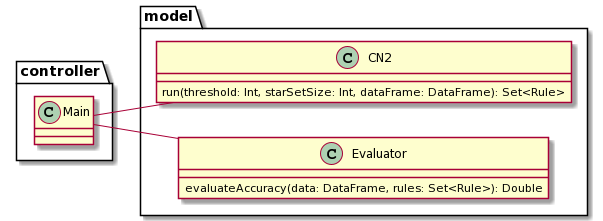
\includegraphics[width=\textwidth]{pictures/main.png}
    \caption{Main structure of the system. CN2 is the effective algorithm implementation while Evaluator allows to evaluate the accuracy of the class inference.}
    \label{figure:main_structure}
\end{figure}

\subsection{Rule, complex and selector}
The output expected from the algorithm is an ordered set of rules. These ones are composed by a complex that is composed of selectors. The selectors can be both numerical and cathegorical. To a graphical representation please refer to Figure \ref{figure:output_types}.
\begin{figure}[ht!]\centering
    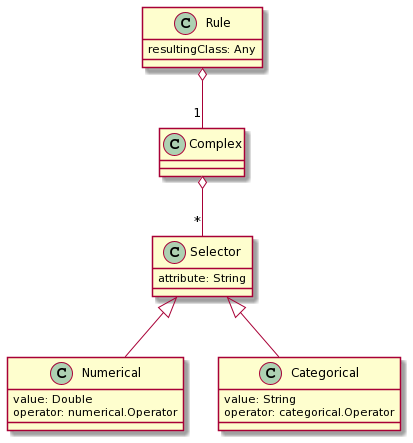
\includegraphics[width=.6\textwidth]{pictures/output_types.png}
    \caption{Types of data relation in the system.}
    \label{figure:output_types}
\end{figure}

\begin{figure}[ht!]\centering
    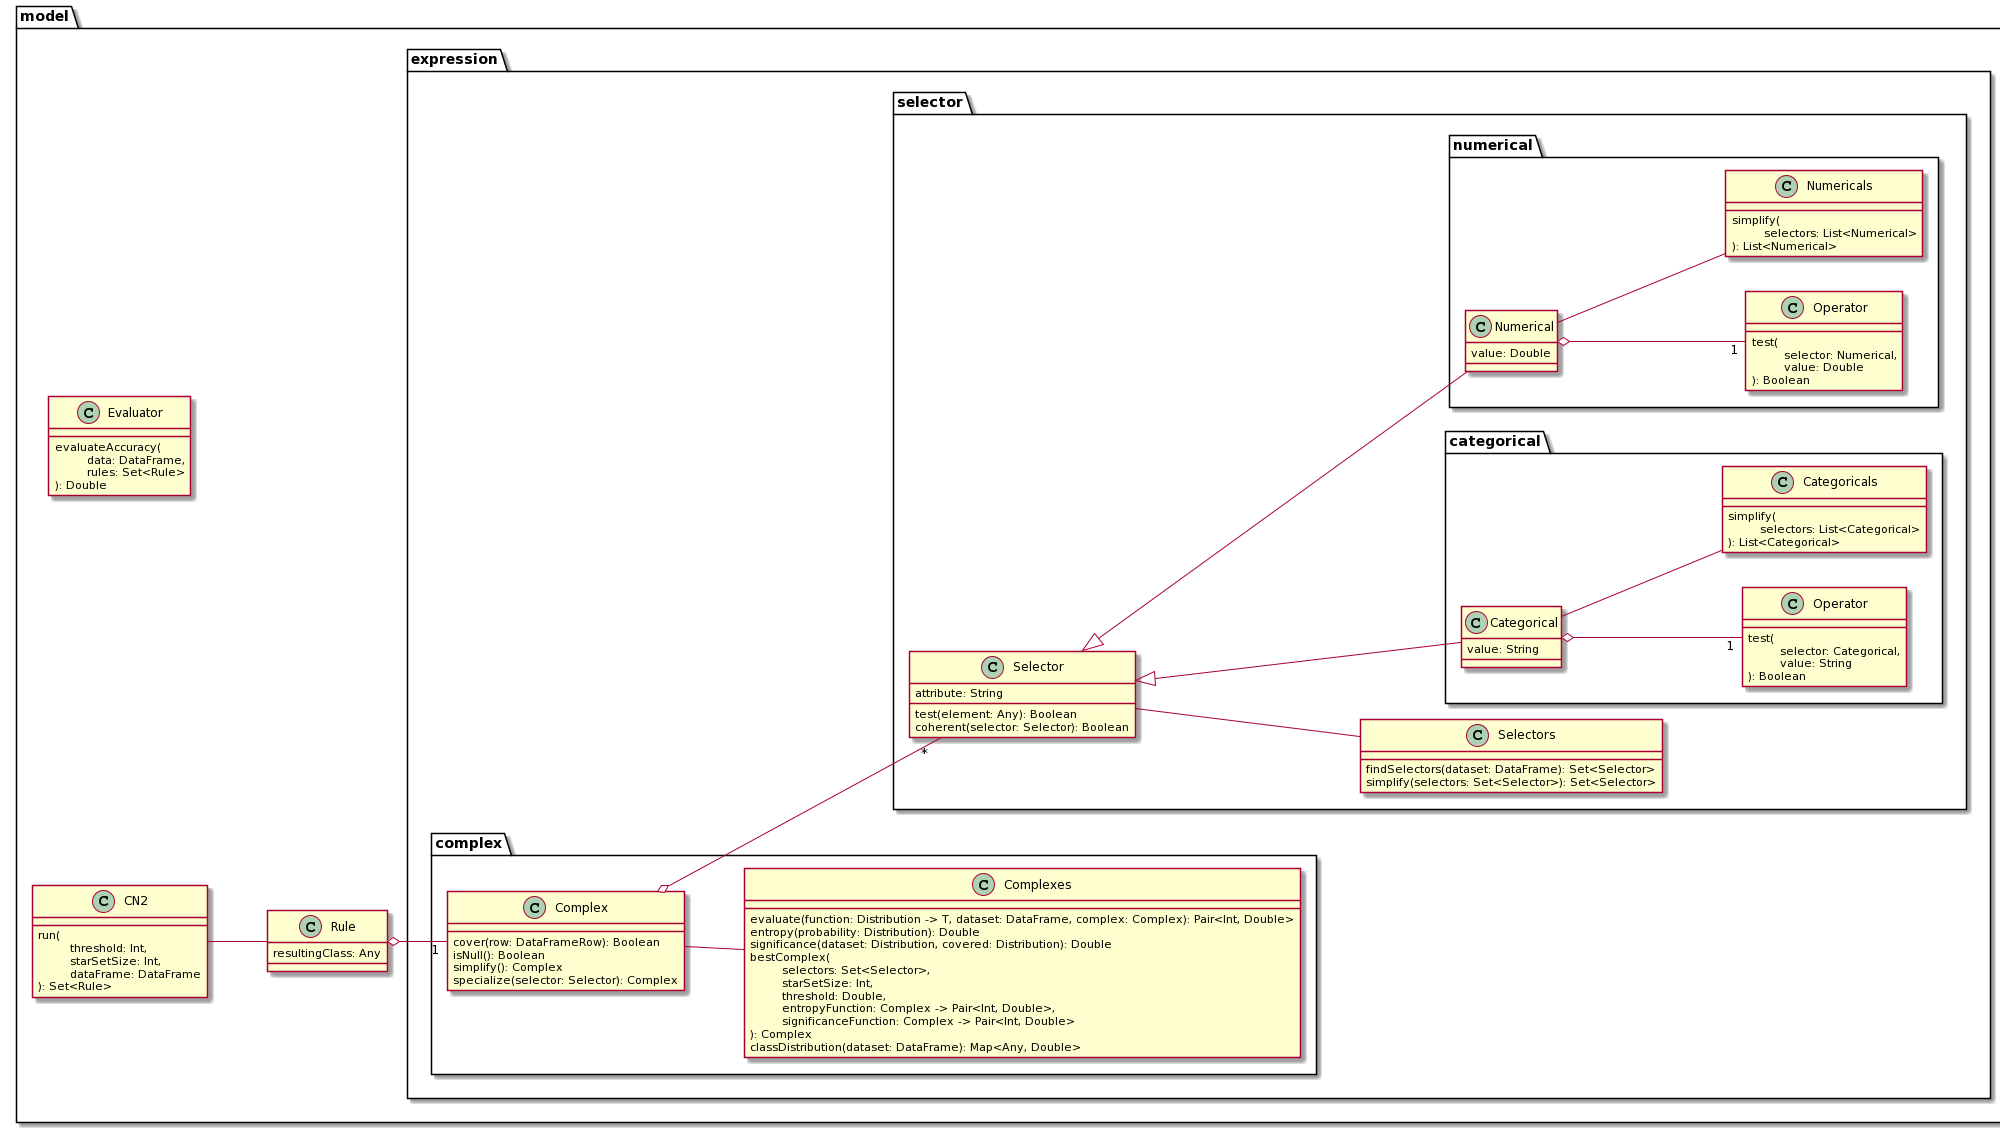
\includegraphics[width=\textwidth]{pictures/model.png}
    \caption{A more complete view of the Model.}
    \label{figure:complete}
\end{figure}
\newpage

%%%%%%%%%%%%%%%%%%%%%%%%%%%%%%%%%%%%%%%%%%%%%%%%%%%%%%%%%%%%%%%%%%%%%%%%%%%%%%%%%%%%%%%%%%%%%%%%%%%
% SECTION 4
%%%%%%%%%%%%%%%%%%%%%%%%%%%%%%%%%%%%%%%%%%%%%%%%%%%%%%%%%%%%%%%%%%%%%%%%%%%%%%%%%%%%%%%%%%%%%%%%%%%

\section{Performed experiments}\label{section:tests}
The experiments were carried on the original datasets used in the paper (converted to the format required by the algorithm: see Section \ref{section:io}).

\subsection{Datasets analysis}
To be able to comprehend the experiments, an initial analysis of the datasets is required.

\paragraph{The breast cancer dataset} includes 201 instances of one class and 85 instances of another class. These instances are described by 9 attributes, some of which are linear and some are nominal. The name and description of each attribute, including its column index in the file, is provided in the following list.
\begin{enumerate}\addtocounter{enumi}{-1}
    \item Class: no-recurrence-events, recurrence-events
    \item age: 10-19, 20-29, 30-39, 40-49, 50-59, 60-69, 70-79, 80-89, 90-99.
    \item menopause: lt40, ge40, premeno.
    \item tumor-size: 0-4, 5-9, 10-14, 15-19, 20-24, 25-29, 30-34, 35-39, 40-44, 45-49, 50-54, 55-59.
    \item  inv-nodes: 0-2, 3-5, 6-8, 9-11, 12-14, 15-17, 18-20, 21-23, 24-26, 27-29, 30-32, 33-35, 36-39.
    \item node-caps: yes, no.
    \item deg-malig: 1, 2, 3.
    \item breast: left, right.
    \item breast-quad: left-up, left-low, right-up,	right-low, central.
    \item irradiat:	yes, no.
\end{enumerate}
The given dataset contains also some missing values. In particular it has 8 missing values for the attribute \textit{deg-malig} (col. 6) and 1 missing value for the attribute \textit{irradiat} (col. 9).
\vspace{12pt}\newline
The accuracy on classification obtained by C\&N with their version of the CN2 algorithm on this dataset belong to the range 65\%-72\%.

\paragraph{The lymphography dataset} includes entries belonging to 4 classes. In particular: 2 belonging to the first class, 81 belonging to the second, 61 belonging to the third and 4 belonging to the fourth. These instances are described by 18 numerical attributes. The name and description of each attribute, including its column index in the file, is provided in the following list.
\begin{enumerate}\addtocounter{enumi}{-1}
    \item class: normal find, metastases, malign lymph, fibrosis
    \item lymphatics: normal, arched, deformed, displaced
    \item block of affere: no, yes
    \item bl. of lymph. c: no, yes
    \item bl. of lymph. s: no, yes
    \item by pass: no, yes
    \item extravasates: no, yes
    \item regeneration of: no, yes
    \item early uptake in: no, yes
    \item lym.nodes dimin: 0-3
    \item lym.nodes enlar: 1-4
    \item changes in lym.: bean, oval, round
    \item defect in node: no, lacunar, lac. marginal, lac. central
    \item changes in node: no, lacunar, lac. margin, lac. central
    \item changes in stru: no, grainy, drop-like, coarse, diluted, reticular, stripped, faint
    \item special forms: no, chalices, vesicles
    \item dislocation of: no, yes
    \item exclusion of no: no, yes
    \item no. of nodes in: 0-9, 10-19, 20-29, 30-39, 40-49, 50-59, 60-69, $>=70$
\end{enumerate}
The given dataset does \textit{not} contain missing values.
\vspace{12pt}\newline
The accuracy on classification obtained by C\&N with their version of the CN2 algorithm (with 99\% threshold) on this dataset is 82\%.

\paragraph{The primary tumor dataset} includes entries belonging to 22 classes. For the distribution of the classes in the data, please refer to the description of the dataset in the \textit{archive.ics.uci.edu} site. These instances are described by 17 numerical attributes. The name and description of each attribute, including its column index in the file, is provided in the following list.
\begin{enumerate}\addtocounter{enumi}{-1}
    \item class: lung, head \& neck, esophasus, thyroid, stomach, duoden \& sm.int, colon, rectum, anus, salivary glands, pancreas, gallblader, liver, kidney, bladder, testis, prostate, ovary, corpus uteri, cervix uteri, vagina, breast
    \item age:   $<30$, 30-59, $>=60$
    \item sex:   male, female
    \item histologic-type: epidermoid, adeno, anaplastic
    \item degree-of-diffe: well, fairly, poorly
    \item bone: yes, no
    \item bone-marrow: yes, no
    \item lung: yes, no
    \item pleura: yes, no
    \item peritoneum: yes, no
    \item liver: yes, no
    \item brain: yes, no
    \item skin: yes, no
    \item neck: yes, no
    \item supraclavicular: yes, no
    \item axillar: yes, no
    \item mediastinum: yes, no
    \item abdominal: yes, no
\end{enumerate}
The given dataset contains also some missing values. In particular it has 1 missing value for the attribute \textit{sex} (col. 3), 67 missing values for the attribute \textit{histologic-type} (col. 4), 155 missing value for the attribute \textit{degree-of-diffe} (col. 5), 1 missing value for the attribute \textit{skin} (col. 13) and 1 missing value for the attribute \textit{axillar} (col. 16).
\vspace{12pt}\newline
The accuracy on classification obtained by C\&N with their version of the CN2 algorithm on this dataset is 36\%.

\paragraph{Credits:} all of this datasets are from the University Medical Centre, Institute of Oncology, Ljubljana, Yugoslavia.

\subsection{Induction with different parameters and considerations}
In this section we will test various combination of initial values to check their influence on the final results. We will then try to draw some consideration on them.\newline
Please consider that the software use multithreading and thus the time required for the rules induction can vary much between different systems. Its use is so just for a qualitative comparison.

\paragraph{Threshold} parameter seems to influence the fitting of the rules over the data. A lower value leaded to overfitting in case of \textit{lymphography} dataset, while it seems to slightly improve the results in the test set of the \textit{primary-tumor}.\newline
This parameter does not seems to affect the induction time of the algorithm.

\begin{center}
    \begin{tabular}{ccccccc}
        Dataset & Threshold & StarSet size & \makecell{Result on\\training set} & \makecell{Result on\\test set} & \makecell{Induction\\time [ms]} & \makecell{Number\\of rules} \\

        primary-tumor & 90 & 5 & 58.15 & 26.88 & 36248 & 105 \\
        primary-tumor & 70 & 5 & 58.15 & 24.73 & 38521 & 109 \\
        primary-tumor & 50 & 5 & 58.15 & 27.96 & 35246 & 104 \\

        lymphography & 90 & 5 & 77.23 & 76.74 & 8521 & 22 \\
        lymphography & 70 & 5 & 85.15 & 74.42 & 11344 & 29 \\
        lymphography & 50 & 5 & 100.00 & 69.77 & 12135 & 24 \\

        breast-cancer & 90 & 5 & 29.15 & 24.71 & 261 & 4 \\
        breast-cancer & 70 & 5 & 29.15 & 24.71 & 132 & 4 \\
        breast-cancer & 50 & 5 & 29.15 & 24.71 & 170 & 4
    \end{tabular}
\end{center}

\paragraph{StarSet size} parameter seems to slightly influence the results on the \textit{primary-tumor} dataset. An higher value requires more computational time but also increased the accuracy of the result in the test set. Moreover, it seems to influence the quantity of rules generated by the algorithm, generating an higher amount when the size is higher. Anyway, it seems to influence less the learning than the threshold parameter.
\begin{center}
    \begin{tabular}{ccccccc}
        Dataset & Threshold & StarSet size & \makecell{Result on\\training set} & \makecell{Result on\\test set} & \makecell{Induction\\time [ms]} & \makecell{Number\\of rules} \\

        primary-tumor & 90 & 15 & 57.27 & 26.88 & 137069 & 107 \\
        primary-tumor & 90 & 10 & 57.27 & 27.96 & 89638 & 109 \\
        primary-tumor & 90 & 5 & 48.90 & 23.66 & 39646 & 95 \\
        primary-tumor & 90 & 1 & 42.73 & 18.28 & 9133 & 78 \\

        breast-cancer & 90 & 15 & 29.15 & 23.53 & 447 & 4 \\
        breast-cancer & 90 & 10 & 29.15 & 23.53 & 140 & 4 \\
        breast-cancer & 90 & 5 & 29.15 & 23.53 & 83 & 4 \\
        breast-cancer & 90 & 1 & 29.15 & 23.53 & 59 & 4 \\

        lymphography & 90 & 15 & 78.22 & 62.79 & 29439 & 25 \\
        lymphography & 90 & 10 & 78.22 & 62.79 & 18204 & 24 \\
        lymphography & 90 & 5 & 78.22 & 62.79 & 6858 & 24 \\
        lymphography & 90 & 1 & 78.22 & 62.79 & 746 & 24
    \end{tabular}
\end{center}

\paragraph{Additional consideration} derived from the given results of the testings is that the accuracy obtained by the algorithm seems more or less good. This is slightly less than the one obtained by C\&N but it can depends on the partition in training and test set.

\newpage

%%%%%%%%%%%%%%%%%%%%%%%%%%%%%%%%%%%%%%%%%%%%%%%%%%%%%%%%%%%%%%%%%%%%%%%%%%%%%%%%%%%%%%%%%%%%%%%%%%%
% SECTION 5
%%%%%%%%%%%%%%%%%%%%%%%%%%%%%%%%%%%%%%%%%%%%%%%%%%%%%%%%%%%%%%%%%%%%%%%%%%%%%%%%%%%%%%%%%%%%%%%%%%%

\section{Conclusion}
From the considerations of Section \ref{section:tests} we can say that the algorithm seems to work sufficiently well. It's accuracy, as already said, is slightly lower than the one obtained by C\&N but it can depend on the subdivision of the datasets in training and test set.\newline
The algorithm is also sufficiently fast, requiring only a bunch of minutes in the worst case.

\newpage

%%%%%%%%%%%%%%%%%%%%%%%%%%%%%%%%%%%%%%%%%%%%%%%%%%%%%%%%%%%%%%%%%%%%%%%%%%%%%%%%%%%%%%%%%%%%%%%%%%%
% SECTION 6
%%%%%%%%%%%%%%%%%%%%%%%%%%%%%%%%%%%%%%%%%%%%%%%%%%%%%%%%%%%%%%%%%%%%%%%%%%%%%%%%%%%%%%%%%%%%%%%%%%%

\section{User guide}
The execution is possible through use of two methods:
\begin{itemize}
    \item Jar file
    \item Gradle automation tool
\end{itemize}

\paragraph{The jar file} will be added to the submission of the project. Through this it is possible to start/use the induction algorithm and the evaluation program. The tool is in a command line interface form and requires to follow the below specified semantic (Listing \ref{listing:semantic}). An example of a valid execution is:
\vspace{6pt}\newline
\texttt{java -jar build/libs/solution-1.0-SNAPSHOT-all.jar res/datasets/lymphography/-\\lymphography.data -v 0 --export}
\begin{lstlisting}[language=bash,label={listing:semantic},caption={Semantic of the CLI program.},captionpos=b]
    Usage: main [OPTIONS] DATASET

    Options:
    -e, --export             Export the inferred rules to file
                             ('rules.dat' by default)
    -o, --output PATH        Path to the file in which save the
                             inferred rules
    -s, --star-set-size INT  Size of the set used to find the best
                             complex. Default 15
    -t, --threshold INT      Minimum level of significance to accept
                             a complex. Default 99
    -v, --verbose-level INT  Level of verbosity during the training
                             (0 is the max level of verbosity)
    -h, --help               Show this message and exit

    Arguments:
    DATASET  Path to the dataset to use for the training
\end{lstlisting}

\paragraph{The Gradle tool} allow to execute the tests and run the program. In the following description some useful commands are described.
\begin{description}
    \item[\texttt{./gradlew test}] run the tests;
    \item[\texttt{./gradlew run --args="ARGUMENTS"}] execute the program passing the \texttt{ARGUMENTS} to it. The arguments should follow the Listing \ref{listing:semantic} semantic;
    \item[\texttt{./gradlew build}] packs the code into a \texttt{NAME-all.jar} file into the \texttt{./build/libs} folder;
\end{description}
An example of a valid execution is:
\vspace{6pt}\newline
\texttt{./gradlew run --args="res/datasets/lymphography/lymphography.data -v 0 --export"}

\end{document}